The Internet of Things paradigm (IoT) fosters the connection of large numbers of sensors to the network. According to Cisco systems~\cite{ciscoGlance}, 500 billion IoT devices are expected to be connected to the Internet by 2030, and mearly 50\% of the data produced worldwide will be generated by IoT sensors~\cite{McAuley}
%
IoT devices produce important and timely data that can lead to new and transformative applications that are important to science and society, such as:
%
\begin{itemize} 
  \item Precision medicine applications that benefit from runtime actuation based on continuous monitoring by scientific instruments.
  \item Urban mobility applications that rely on processing data from sensors to identify and alleviate traffic congestion. 
  \item Healthcare applications that infer lifestyle patterns based on behavioral information obtained from wearables. 
\end{itemize} 

Making such applications a reality requires collecting data from sensors and instruments, processing this data individually or collectively in a timely manner, and making decisions based on the results. 

Stream processing frameworks (SPFs) have proven to be very effective at processing large amounts of data at near-real-time, especially when combined with the elasticity and scalability of the cloud. Nonetheless, existing solutions were developed keeping in mind Big Data streams generated at the core of the infrastructure, such as those associated with web analytics. As a result, applying these solutions to IoT data stream requires transferring data from the edges to a data center located at the core of the infrastructure for processing. This model of moving data is quickly becoming unsustainable~\cite{intro}, due to the resulting impact on latency, network congestion, storage cost, and privacy, limiting the potential impact of IoT.

However, in recent years, non-trivial computational capabilities have proliferated across the computing service landscape~\cite{continuum}. In particular, edge services are emerging closer to the data sources and can provide potential data-processing capabilities\cite{dastjerdi2016fog,bonomi2014fog}. 

Edge computing extends the conventional centralized cloud infrastructures with an additional storage and processing layer that enables execution of application logic close to end-user. Edge computing foresees the deployment of edge nodes, which may range from IoT embedded devices featuring limited storage, memory, and processing capacity to whole data centers (i.e. "local clouds") which are deployed closer to end-users and physical infrastructures. Overall, the edge computing paradigm extends the cloud paradigm to the edge of the network. In this way, users can benefit from computing, storage and communication resources at their vicinity, instead of interfacing to a centralized back-end cloud. The proximity of resources helps to overcome the high-latency that is associated with the provision of cloud services to mobile users.

IoT data feature certain characteristics, which distinguish them radically from other types of data sources and respective applications. The special characteristics and related challenges for IoT data processing applications can be listed as follows:

\begin{itemize}

\item{\textbf{Geographically Distributed:}} IoT data streams are produced in a geographically distributed fashion manner.

\item{\textbf{Time and Location:}} The data streams contains temporal and spatial dependencies, which are directly related with the value. For that reason IoT applications need to process data in a timely fashion and from the proper location, in order to extract its maximum value.

\item{\textbf{Real-Time:}} IoT data streams are produced in high velocities (machine speed) and requires applications to process the data in real-time. 

\item{\textbf{Security:}} The majority of the IoT data produced by sensors contains personal and sensitive data.

\item{\textbf{Mobility:}} IoT applications can involve sensors that moves around such as: connected vehicles, autonomous cars, etc... and requires the communication to local resources (computing, storage) residing in their vicinity. 

\end{itemize}

While edge computing can help achieve all the new requirements that IoT applications need, edge resources are typically constrained in their capabilities. Therefore, edge computing can be leveraged to complement the computing capabilities of the cloud-centric approach. The use of edge and cloud architecture poses several challenges: 

\begin{itemize}
\item Deciding how to split IoT applications among the edge and cloud resources, in order to meet the requirement of the application; Where an IoT application is a sequence of operators from a source to a sink. 

\item Exploring heterogeneous infrastructure for deploying data flow applications has proved to be NP-hard~\cite{Benoit:2013}. Due to the fact that there are so many possible combinations (many edge devices and many operators to place). 
 
\item Moving operators from cloud to edge devices is challenging due to the devices' limitations with respect to memory, CPU, and often network bandwidth \cite{dias:2018:survey}.
\end{itemize}

Solving the challenges presented above in a correct manner will allow for faster completion time, a reduction in edge to cloud data transfers, and ensure efficient use of the edge and cloud resources. Doing them incorrectly can be detrimental to throughput and exacerbate the time for handling data events.
 
\section{Motivation}

The popularity and proliferation of the Internet of Things (IoT) paradigm is resulting in a growing number of devices connected to the Internet. These devices are generating and consuming unprecedented amounts of data at the edges of the infrastructure, and are enabling new classes of applications, however, current approaches typically rely on cloud platforms located at the core of the infrastructure to process data. As the number of devices and the amount of data they generate and consume increases, such core-centric approaches are becoming increasingly inefficient as they need to transfer data back and forth between the edge and the core. Furthermore, not all the data produced is interesting or relevant, and only a part of it may need to be processed in the context of an application. These observations can be leveraged to design hybrid architectures that can effectively leverage both the edge and the cloud resources to process the data in an effective and timely manner\cite{ahmed2017role, satyanarayanan2015edge}.

To address these limitations, we propose R-Pulsar, a software stack with a content- and location-based programming abstraction to perform and orchestrate data analytics between the edge and the cloud. The programming abstraction enables developers to address the \textbf{what}, \textbf{where}, and \textbf{when} data needs to be processed by specifying content and action descriptors. We also propose a programming model to provide developers with the ability to define \textbf{how} to automatically split the dataflow across the edge and the cloud by specifying a set of dataflow constraints. In addition we present an optimized data-processing pipeline for achieving real-time data analytics on constrained devices.

\section{Problem Description}

With the increasing number of connected IoT devices, providing efficient and effective streaming analytics across the edge and the cloud for IoT applications is non-trivial due to the characteristics of IoT streams.
\\\\
\noindent\textbf{What data to consume}
\\
Due to the large number of IoT devices/sensors that are currently online, not all the data produced by the sensors is interesting or relevant, or only a part of it may need to be
processed in the context of an application. Requiring all the data to be transported to the
cloud for processing, will result in latencies that can prevent timely decision making or may reduce the amount of data processed. As a result there is a need for a programming model to help developers decide what data they want to consume.
\\\\
\noindent\textbf{Where to perform the computations}
\\
As mentioned earlier IoT streams have time and location dependencies, so in order to satisfy the requirements, computations needs to be placed between the edge and the cloud. Due to the hardware heterogeneity of edge and cloud resources, there is a need for a programming model that allows developers to reason about where they want the computations to be placed. Since edge resources are typically constrained in their capabilities and cloud resources are suited to perform heavier (resource intensive) analysis.
\\\\
\noindent\textbf{When to perform computations}
\\
Edge computing helps reduce the latency and the total amount of data and the load that is sent to the cloud by pre-processing, filtering and analyzing at the edge of the network. Once the data is pre-processed at the edge of the network a decision need to be made to either discard it or forward it to the cloud for post-processing. For those reasons there is a need for a rule programming abstraction to allow the ability to decide when and where to perform post-processing computations.
\\\\
\noindent\textbf{How to split IoT applications across the edge and the cloud}
\\
Cloud-based architectures often centralize storage and processing, generating high data
movement overheads that penalize real-time applications. Edge and Cloud architecture pushes computation closer to where the data is generated, reducing the cost of data movements and improving the application response time. The heterogeneity among the edge devices and cloud servers introduces an important challenge for deciding how to split and orchestrate the IoT
applications across the edge and the cloud. For those reasons there is a need for a programming model to provide developers with the ability to define how to automatically split the dataflow across the edge and the cloud by specifying a set of dataflow constraints.

\section{Contributions}
The primary contributions of the research in this thesis are a programming model for deciding \textbf{what}, \textbf{when}, \textbf{where} data needs to be processed by specifying content and action descriptors and \textbf{how} computations get distributed across the edge and the cloud. The detailed contributions are presented as follows.
\begin{itemize}
  \item A content- and location-based programming abstraction for specifying \textbf{what} data gets collected and \textbf{where} the data gets analyzed.
  \item A rule-based programming abstraction for specifying \textbf{when} to trigger data-processing tasks based on data observations.
  \item A programming abstraction for specifying \textbf{how} to split a given dataflow and place operators across edge and cloud resources.
  \item An operator placement strategy that aims to minimize an aggregate cost which covers the end-to-end latency (time for an event to traverse the entire dataflow), the data transfer rate (amount of data transferred between the edge and the cloud) and the messaging cost (number of messages transferred between edge and the cloud).
  \item Performance optimizations on the data-processing pipeline in order to achieve real-time performance on constrained devices.
  \item An implementation of the above capabilities as part of the R-Pulsar software stack and its evaluation using embedded devices (Raspberry Pi and Android phone).
\end{itemize}

\section{Outline}

\begin{figure}[h!]
  \centering
  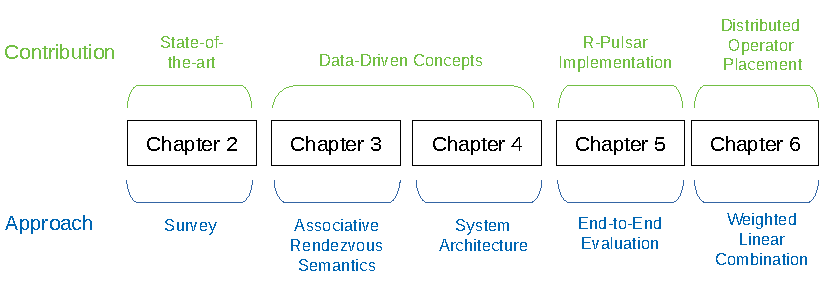
\includegraphics[width=1\textwidth]{Figures/Outline.pdf}
  \caption{Thesis Organization.}
  \label{fig:Outline}
\end{figure}

The core chapters of the thesis are structured as shown in Figure~\ref{fig:Outline} and are deviated from articles and journals published during the PhD. The remaining of the thesis is organized as follows: 

\begin{itemize}
    \item Chapter 2 shows some of the IoT application that where used in order to motivate and validate the build of R-Pulsar.  
    \item Chapter 3 presents an extensive literature review of all the commercial and academic edge-based middleware currently available. 
    \item Chapter 4 presents the Associative Rendezvous programming abstraction that R-Pulsar builds upon.
    \item Chapter 5 presents the system concepts and all the layers on what R-Pulsar was build upon. 
    \item Chapter 6 presents the implementation and evaluation details of all the layers that R-Pulsar consists. 
    \item Chapter 7 introduces the operator placement problem, to solve the how to split IoT applications dynamically across the edge and the cloud. 
    \item Chapter 8 concludes the dissertation by outlining future research work.
\end{itemize}

